\documentclass[9pt, compsoc, journal]{IEEEtran}
\usepackage[utf8]{inputenc}
\usepackage{graphicx}
\graphicspath{ {./_figures/} }
\usepackage{multicol}
\bstctlcite{IEEEexample:BSTcontrol}
\usepackage{bigstrut}
\usepackage{multirow}
\usepackage{tabularx}
\usepackage{tabulary}
\usepackage{booktabs}
\usepackage{fullpage}
\usepackage{amsmath}
\usepackage{bookman}
\usepackage{balance}
\usepackage{flushend}
\usepackage[caption=false,font=normalsize,labelfont=sf,textfont=sf]{subfig}
\usepackage{hyperref}
\hypersetup{colorlinks = False}
\usepackage[english]{babel}
\usepackage{blindtext}
\usepackage{times}
\usepackage{cite}
\hypersetup{colorlinks,breaklinks,
            urlcolor=[rgb]{0,0,0},
            citecolor=[rgb]{0,0,0},
            linkcolor=[rgb]{0,0,0}}
\usepackage{fullpage}
\linespread{1}
\usepackage[table]{xcolor}
\linespread{0.99}

\begin{document}
  
  \title{A Case for Multi-Objective Search in Automated Patch Generation}
  \author{Rahul Krishna, 
  \IEEEauthorblockA{\normalsize {\textit{Department of Computer Science}\\
    North Carolina State University, Email: 
    \href{mailto:rkrish11@ncsu.edu}{{rkrish11@ncsu.edu}}}}}

\maketitle
\section{Motivation}

Automated Patch generation has garnered a lot of attention in the past decade. Specifically, tools like GenProg have seen tremendous success. In fact, GenProg is now used as a baseline to compare other new techniques. Albeit popular, there is a general lack of agreement on the need for complex tools like GenProg to generate effective patches. While some researchers~\cite{leGoues12} opine that GenProg is quite effective in generating patches, given the existence of test cases, others \cite{qi2014, kim2013, arcuri2011} disagree. They say that it is quite unclear if the the efficacy of GenProg is merely due to its ``mutate'' operator or due to genetic programming.

This issue was examined by Qi et at.~\cite{qi2014}. With their tool RSRepair (\underline{\textit{R}}andom-\underline{\textit{S}}earch \underline{\textit{Repair}}), they demonstrated the benefit of random search over GenProg. 

It is my hypothesis that the lack of efficiency of GenProg in this area is not due to the failure of Genetic Algorithms (or any evolutionary computation scheme for that matter), but due to incorrect and perhaps even incomplete modeling of the search space.

As a motivating example consider Genetic Programming. The algorithm works by trying to maximize the ``fitness'' score. In this case, the number of passing test cases given a patch. RSRepair, on the other hand, considers either repair effectiveness (as measured by the number patch trials required) or repair efficiency (measured by the number of test case executions). It not hard to see that each of these objectives namely, the number of passing test cases, the repair effectiveness, and the repair efficiency, are all important. Perhaps some are more important than others, but they all play a crucial role nonetheless.

Therefore, I conjecture that the research in the area of automated patch generation will be best guided by modeling the domain as a multiobjective search problem with the aforementioned objectives. This, in my opinion, will allow us to leverage the wealth of research in Search Based Software Engineering (referred to henceforth as \textit{SBSE}). To this end, this project asks the following two research questions:

\subsubsection*{RQ1: Can automated patch generation be modeled as a multiobjective search problem?}
Although it makes theoretical sense to view patch generation as containing multiple objectives, this question asks if it is practical to model it as such.

\subsubsection*{RQ2: If yes, what is the best multiobjective search to generate patches automatically?}
\label{rq2}
If the answer to RQ1 is affirmative. This question aims to explore various multiobjective optimizers to identify the best algorithm. Specifically, this project will compare three standard SBSE techniques: NSGAII, MOEAD, Genetic Programming, using Random Search as a baseline. In addition to this, the usefulness of a promising new algorithm called SWAY\footnote{This algorithm is in current development by our research group (see \href{http://ai4se.net}{{http://ai4se.net}}).}~\cite{chen2016sampling, nair2016accidental} will be also be investigated. 

\section{An Overview of Patch Generation}

Generally, when a bug is reported, an automated program repair scheme undertakes the following three steps:

\begin{enumerate}
    \item \textit{Fault localization:}
    These techniques are used to identify suspicious faulty code snippet that may a have caused the bug.
    
    \item \textit{Patch Generation:}
    Once faulty code snippet has been located, many candidate patches can be generated through the modifications to that code snippet, according to specific repair rules based on either evolutionary computation or code-based contracts. 
    
    \item \textit{Patch Validation:}
    When a candidate patch has been produced, regression testing, inclusive of negative test cases (reproducing the fault) and positive test cases (characterizing the normal behaviors), is commonly used to validate the correctness of produced candidate patch.

\end{enumerate}

The above procedure can be iterated over and over again until some valid patch is found. Any patch passing all these test cases is considered valid. 

\begin{figure}[!tb]
    \resizebox{1.01\linewidth}{!}{
		\begin{tabular}{ll}
			\hline
			\rowcolor[HTML]{EFEFEF} 
			\multicolumn{1}{l}{\cellcolor[HTML]{EFEFEF}{\bf Measure}} & \multicolumn{1}{c}{\cellcolor[HTML]{EFEFEF}{\bf  Description}}  \\ \hline
			\rowcolor[HTML]{FFFFFF} 
			{\bf Runtime}  & \begin{tabular}[l]{@{}l@{}}Time taken for the algorithm to be gener-\\ate optimal solutions.\end{tabular}\\\hline
			\rowcolor[HTML]{FFFFFF} 
			{\bf Speed Up}  & \begin{tabular}[l]{@{}l@{}}Ratio of time taken for the parallelized \\ version of the algorithm over the time\\taken for the serial version.\end{tabular}\\\hline
			\rowcolor[HTML]{FFFFFF} 
			{\bf Convergence}  & \begin{tabular}[l]{@{}l@{}}Convergence represents the accuracy of \\the obtained solutions. It is the distance\\between the obtained solutions and ideal\\Pareto frontier.\end{tabular}\\\hline
			\rowcolor[HTML]{FFFFFF} 
			\hline{\bf Diversity}                                           & \begin{tabular}[l]{@{}l@{}}Diversity represents the spread of the\\proposed solutions. Ideally the solutions\\should be well distributed across the Par-\\eto frontier,rather than concentrated in\\certain regions.\end{tabular}\\ \hline
		\end{tabular}}
		\caption{Performance Measures}
		\label{fig:measure}
	\end{figure}
\section{A (very) Brief Overview of Multiobjective Search}

A search is the task of finding one or more solutions which satisfy one or more specified objectives. While a single-objective optimization involves a single objective function and a single solutions, a multiobjective optimization considers several objectives simultaneously. In reference to the current problem we have three competing objectives, all of which need to be maximized: (1) Number of passing test cases; (2) The repair effectiveness; and (3) The repair efficiency 

In such a case, a multiobjective optimizer generates a set of alternate solution with certain trade-offs. These are called \textit{Pareto Optimal Solutions}. The solutions, in our case, will be a set of valid patches that perform equally well when measured in terms of the three objectives.

Multiobjective problems are usually complex, NP-Hard, and resource intensive. Although exact methods can be used, they consume prohibitively large amounts of time and memory. An alternative approach would be to make use of metaheuristic algorithms from RQ2. These approximate the Pareto frontier in a reasonable amount of time. 

\section{Evaluation}

\begin{figure}[bt!]
\centering
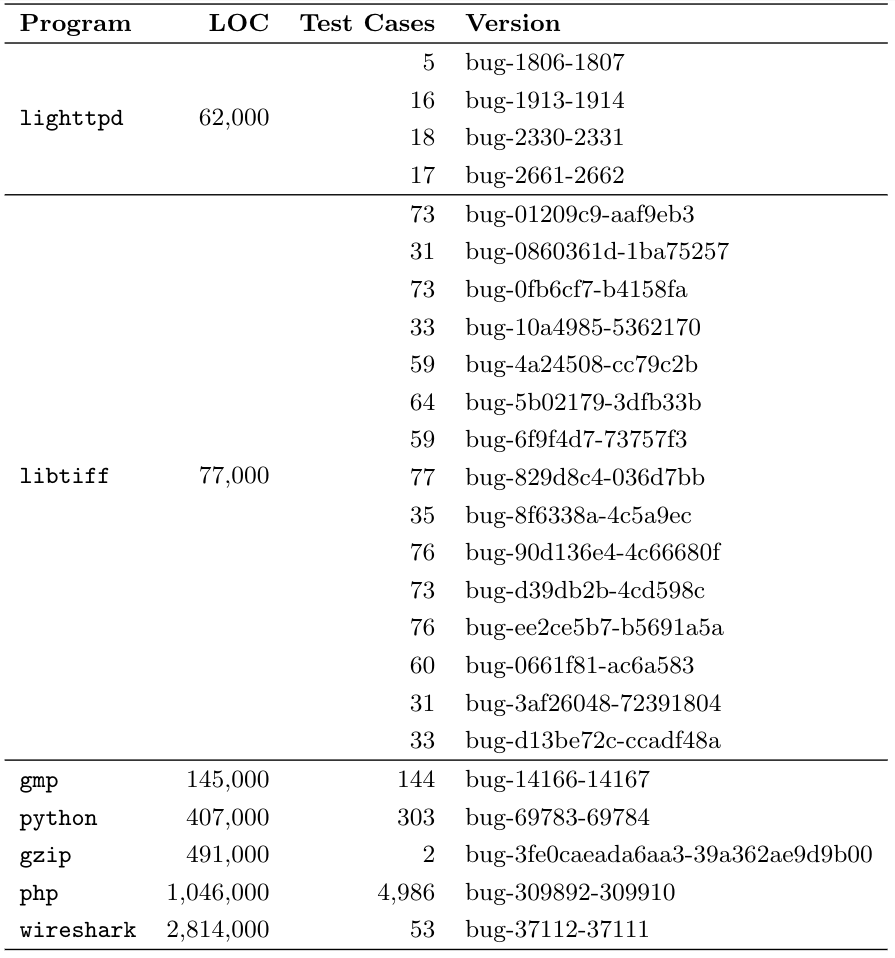
\includegraphics[width=\linewidth]{datasets.png}
\caption{Subject Programs. Image courtesy~\cite{qi2014}.}
\label{fig:datasets}
\end{figure}
\begin{figure}[b!]
\resizebox{1.01\linewidth}{!}{
\begin{tabular}{|
>{\columncolor[HTML]{EFEFEF}}c |l|l|}
\hline
\cellcolor[HTML]{C0C0C0}\textbf{Milestone} & \multicolumn{1}{c|}{\cellcolor[HTML]{C0C0C0}\textbf{Task}} & \multicolumn{1}{c|}{\cellcolor[HTML]{C0C0C0}\textbf{Timeline}} \\ \hline
\textbf{1} & Setup problem domain: Get and verify datasets & 10/18/16 \\ \hline
\textbf{2} & Create a python package that implements the five algorithms & 10/28/16 \\ \hline
\cellcolor[HTML]{EFEFEF} &  &  \\
\multirow{-2}{*}{\cellcolor[HTML]{EFEFEF}\textbf{3}} & \multirow{-2}{*}{\begin{tabular}[c]{@{}l@{}}Establish fitness measurements on the dataset. This maybe\\ a tedious task and my take the longest time.\end{tabular}} & \multirow{-2}{*}{11/18/16} \\ \hline
\textbf{4} & Generate Pareto Optimal solutions and run validations & 11/21/16 \\ \hline
\cellcolor[HTML]{EFEFEF} &  &  \\
\multirow{-2}{*}{\cellcolor[HTML]{EFEFEF}\textbf{5}} & \multirow{-2}{*}{\begin{tabular}[c]{@{}l@{}}Assess results in terms of the Research Questions and prepare\\ a report.\end{tabular}} & \multirow{-2}{*}{11/25/16} \\ \hline
\end{tabular}}
\caption{Timeline}
\label{time}
\end{figure}

\subsection{Metrics}
Figure \ref{fig:measure} highlights some of the preliminary performance evaluation measures we use to evaluate the algorithms. Please note that this will be expanded in future to accommodate other measures.

\subsubsection{How to calculate them?}
Calculating these metrics are well studied~\cite{deb2002fast, goel2010study}. We have an implementation in place that can readily give these metrics, given a set of ideal solutions (in this case, valid patches).

\subsection{Datasets}
The data set required for evaluating will be obtained from some recent work on GenProg~\cite{leGoues12}. My reading of the literature suggests that these dataset are the ``benchmarks'', used by several researchers~\cite{qi2014}. These are C programs with all the bugs reported reported in the historical versions as tabulated in Figure~\ref{fig:datasets}.

\subsection{Tools}
As for tools, it is worth noting that AST can be generated from C programs using a tool called CIL\footnote{https://sourceforge.net/projects/cil/}.  

\subsection{Analysis Plan}
To provide a more comprehensive comparison, the optimizers will be ranked ranked statistically. To do this, I shall use the Scott-Knott procedure recommended by Mittas \& Angelis\cite{mittas13}. 

This method sorts a list of $l$ treatments with $ls$ measurements by their median
score. It then
splits $l$ into sub-lists $m,n$ in order to maximize the expected value of
differences  in the observed performances
before and after divisions. E.g. for lists $l,m,n$ of size $ls,ms,ns$ where $l=m\cup n$:
\[E(\Delta)=\frac{ms}{ls}abs(m.\mu - l.\mu)^2 + \frac{ns}{ls}abs(n.\mu - l.\mu)^2\]
Scott-Knott then applies some statistical hypothesis test $H$ to check
if $m,n$ are significantly different. If so, Scott-Knott then recurses on each division.



\section{Proposed Timeline}

Figure \ref{time} highlights the proposed timeline for the tasks undertaken in the project. Please note again that this subject to change, please see \href{https://github.com/ai-se/spatch/milestones}{{https://github.com/ai-se/spatch/milestones}} for the latest milestone progress.\\
\pagebreak
\bibliographystyle{unsrt}
\bibliography{References}
\end{document}
